\documentclass[no]{./../../common/SurferDesc}%%%%%%%%%%%%%%%%%%%%%%%%%%%%%%%%%%%%%%%%%%%%%%%%%%%%%%%%%%%%%%%%%%%%%%%
%
% The document starts here:
%
\begin{document}
\footnotesize
% Weltrekordfl�chen

%%% 1.Tafel

%%%%%%%%%%%%%%%%%%%%%%%%%%%%%

\begin{surferPage}
  \begin{surferTitle}Cayley-flaten av tredje grad\end{surferTitle}  \\
Denne flaten av tredje grad har fire singulariteter. Den har f�tt navn etter Arthur Cayley, som forsket mye p� slike flater p� 1800-tallet.
    
    Det var imidlertid Ludwig Schl�fli som f�rst klassifiserte disse flatene i 1863. Han systematiserte dem etter hvilke typer singulariteter flatene kunne ha
	For eksempel kan man i artikkelen hans lese om hvorfor det ikke kan v�re mer enn $4$ singul�re punkter p� en flate av tredje grad
    det vil si at: $\mu(3)=4$. 
    
Rundt 1900 studerte Felix Klein de mulige formene til reelle flater av tredje grad. Hans l�sning var � starte med Cayley-flaten av tredje grad og legge sm� deformasjoner til denne: Ved � trekke fra hverandre eller f�re sammen de doble kjeglene, kunne han finne alle de mulige formene som flater av tredje grad kan ha. Her er noen av dem: 
    \vspace{0.3cm}
     \begin{center}
      \vspace{-0.2cm}
      \begin{tabular}{@{}c@{\ }c@{\ }c@{\ }c@{}}
        \begin{tabular}{@{}c@{}}
          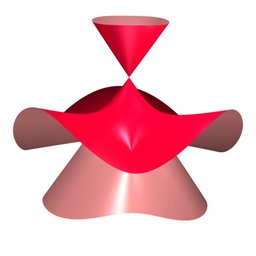
\includegraphics[width=1.35cm]{./../../common/images/cayley_cubic_0}
        \end{tabular}
        &
        \begin{tabular}{@{}c@{}}
          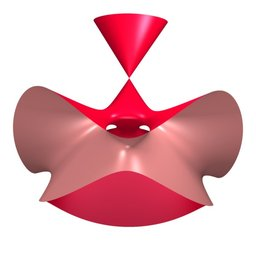
\includegraphics[width=1.35cm]{./../../common/images/cayley_cubic_1}
        \end{tabular}
        &
        \begin{tabular}{@{}c@{}}
          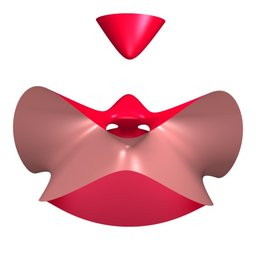
\includegraphics[width=1.35cm]{./../../common/images/cayley_cubic_2}
        \end{tabular}
        &
        \begin{tabular}{@{}c@{}}
          
\includegraphics[width=1.35cm]{./../../common/images/cayley_cubic_3}
        \end{tabular}
      \end{tabular}
    \end{center}

  \begin{surferText}
     \end{surferText}
\end{surferPage}

%%%%%%%%%%%%%%%%%%%%%



\end{document}
%
% end of the document.
%
%%%%%%%%%%%%%%%%%%%%%%%%%%%%%%%%%%%%%%%%%%%%%%%%%%%%%%%%%%%%%%%%%%%%%%%
